\section{Computer Vision}
Computer Vision is a field of Artificial Intelligence and Computer Science that aims at giving computers a visual understanding of the world.

The goal of Computer Vision is to emulate human vision using digital images through three main processing components, executed one after the other:
\begin{itemize}
    \item Image acquisition.
    \item Image processing.
    \item Image analysis and understanding.
\end{itemize}
\begin{figure}[H]
\centering
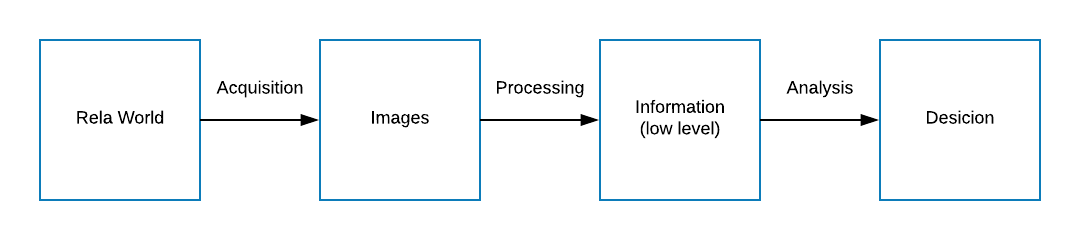
\includegraphics[width=10cm,height=10cm,keepaspectratio]{imagenes/ComputerVisionBlocks.png}
\caption{Computer Vision work flow}
\label{fig:ComputerVision}
\end{figure}
As the human visual understanding of world is reflected in the ability to make decisions through what humans see, providing such a visual understanding to computers would allow them the same capabilities.

\subsection{Image acquisition}
Image acquisition is the process of translating the analog data into binary data. interpreted as digital images.
Different tools have been created to build such data sets:
\begin{itemize}
    \item Webcams and embedded cameras.
    \item Digital compact cameras and DSLR.
    \item Consumer 3D cameras and laser range finders.
\end{itemize}
Most of the time, the raw data acquired by these devices needs to be post-processed in order to be more efficiently exploited in the next steps.

\subsection{Image processing}
The second component of Computer Vision is the low-level processing of images. Algorithms are applied to the binary data acquired in the first step to infer low-level information on parts of the image. This type of information is characterized by image edges, point features or segments, for example.

This second step usually involves advanced applied mathematics algorithms and techniques.

Low-level image processing algorithms include:
\begin{itemize}
    \item Edge detection.
    \item Segmentation.
    \item Classification.
    \item Feature detection and matching.
\end{itemize}

\subsection{Image analysis and understanding}
The last step of the Computer Vision pipeline is the actual analysis of the data, which will allow the decision making.
High-level algorithms are applied, using both the image data and the low-level information computed in previous steps.

Examples of high-level image analysis are:
\begin{itemize}
    \item 3D scene mapping.
    \item Object recognition.
    \item Object tracking.
\end{itemize}
\subsection{Applications of computer vision}
Techniques developed for computer vision have many application in the fields of robotics, human-computer interaction and visualization, to name a few.
\begin{enumerate}
    \item Motion recognition.
    \item Augmented reality.
    \item Autonomous cars.
    \item Domestic robots.
    \item Image restoration.
\end{enumerate}
